% 3.method.tex - EATA Methodology
\section{Methodology}
\label{sec:method}

This section presents the technical details of the Explainable Algorithmic Trading Agent (EATA). We first establish a unified notation system summarized in Appendix~\ref{app:notation}, then describe the core algorithms with their design rationale.

\begin{figure*}[htbp]
\centering
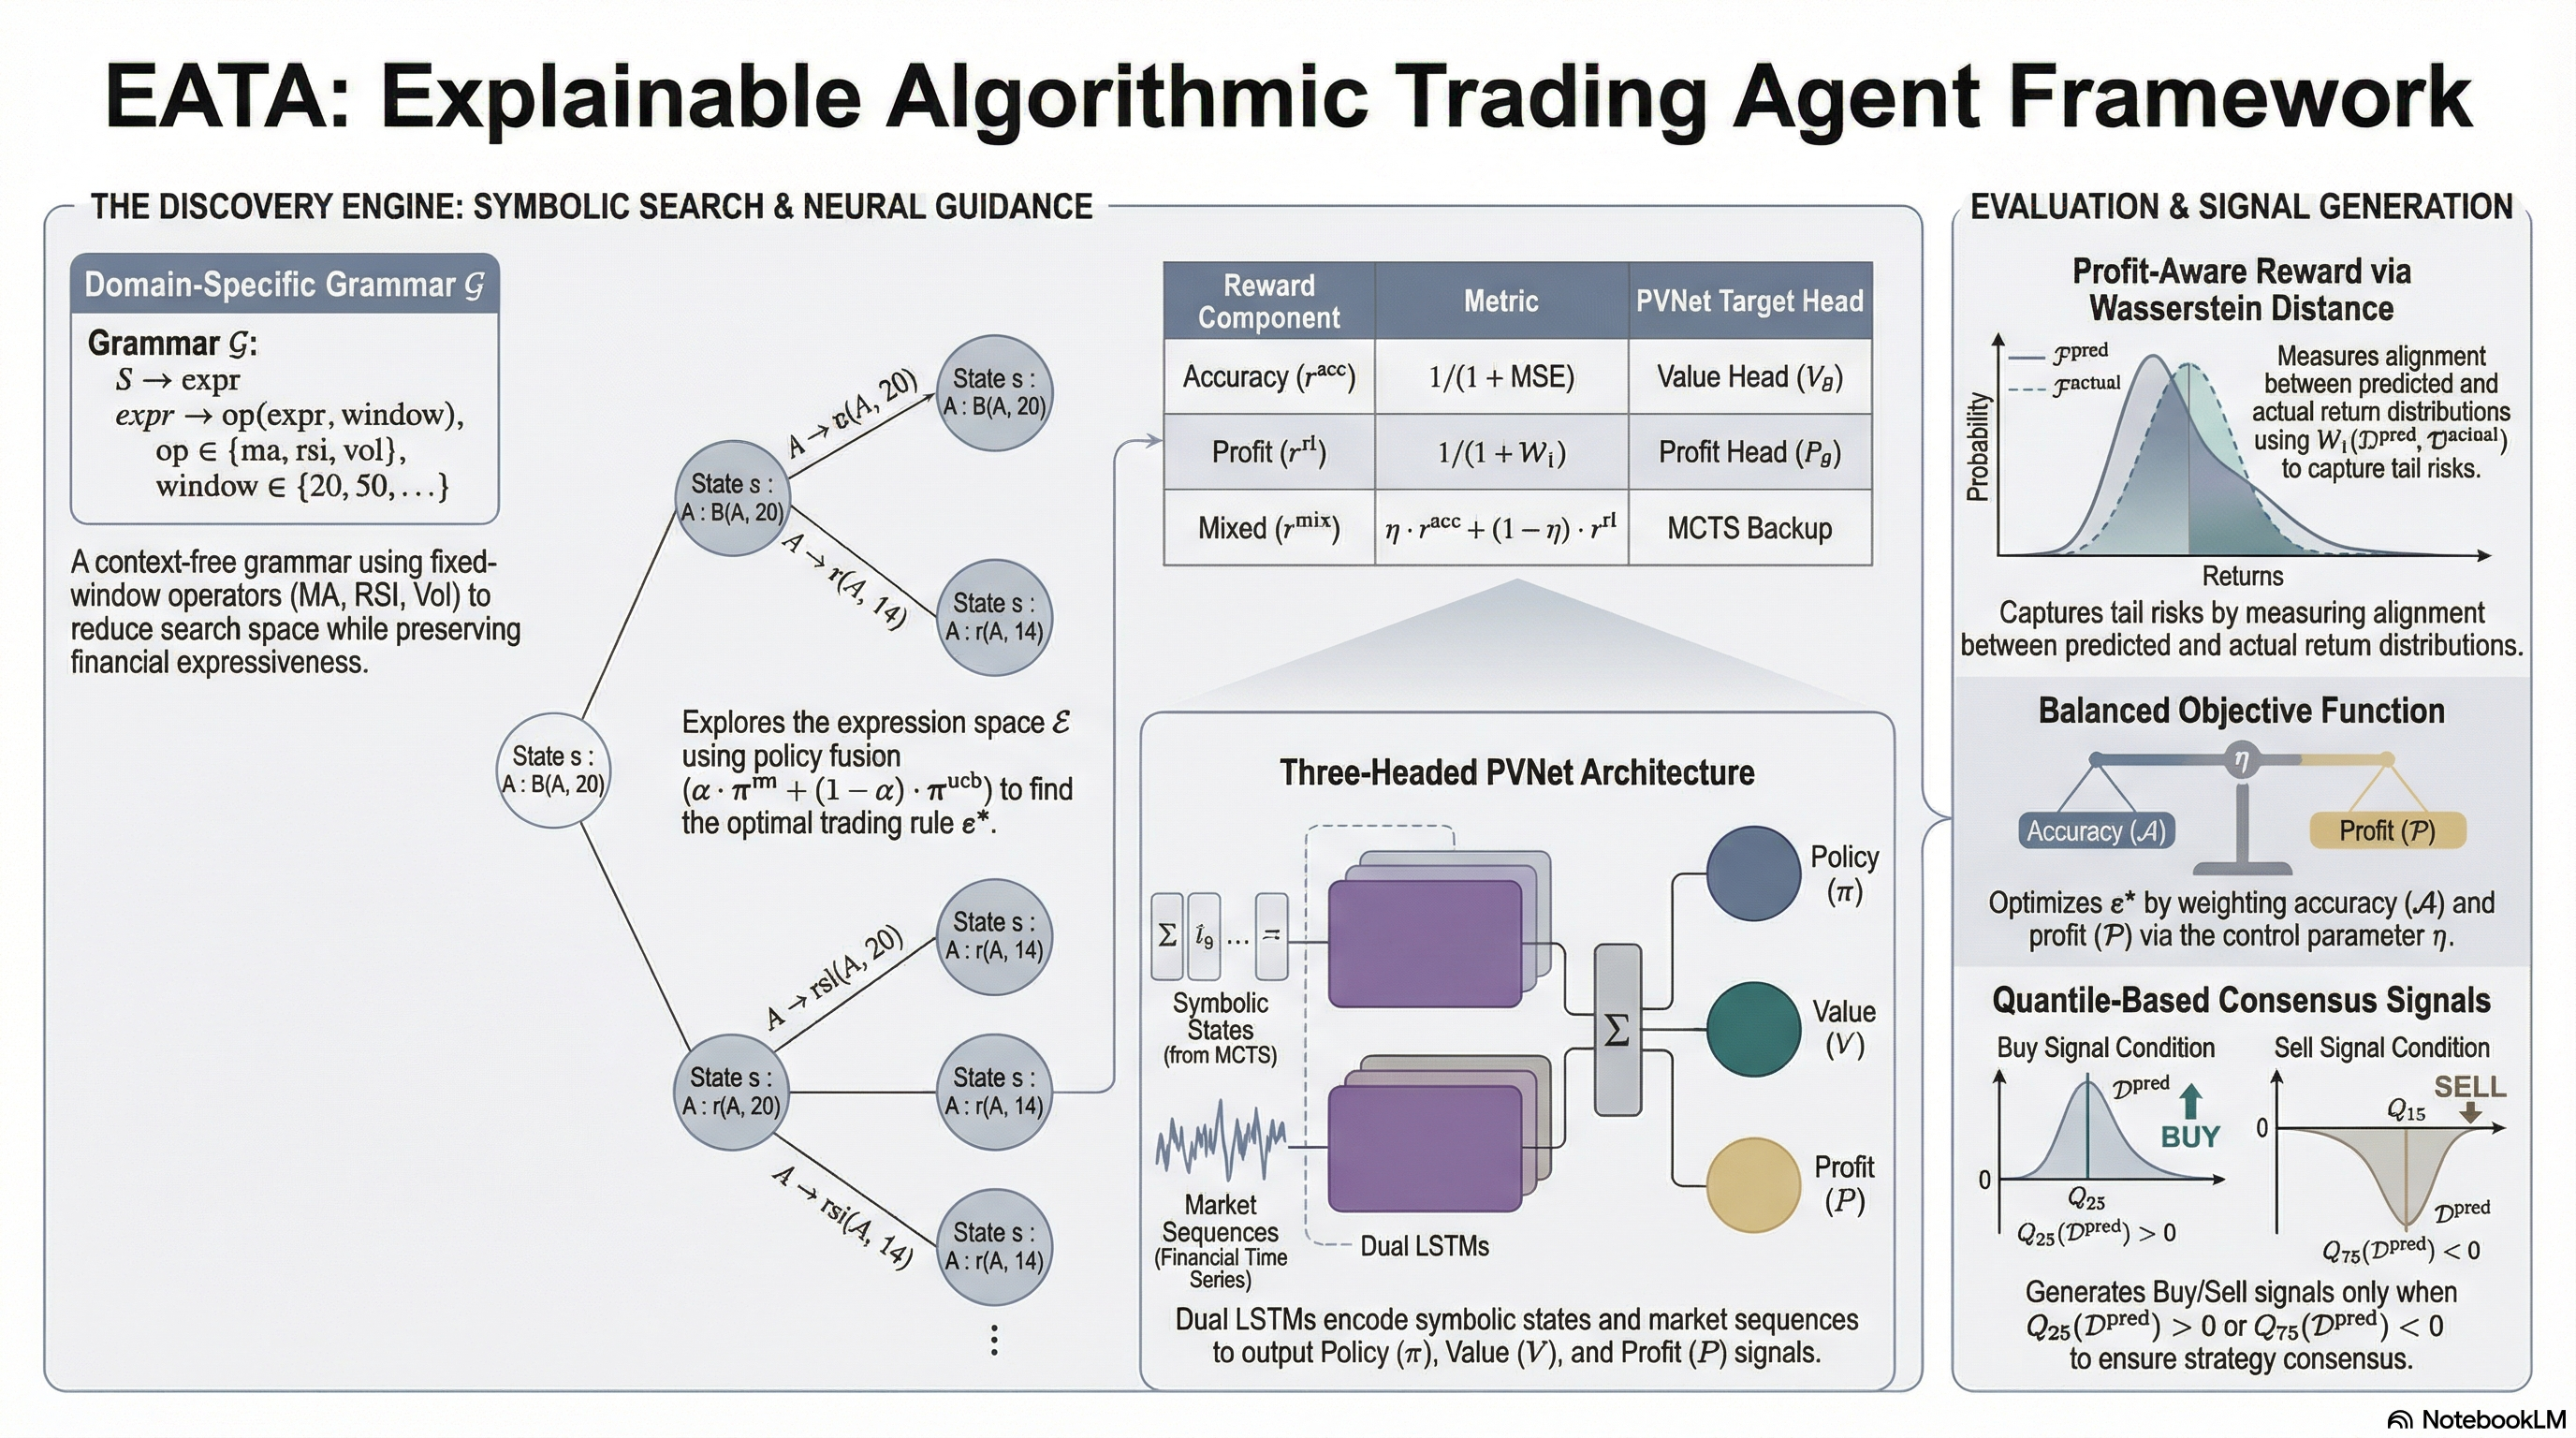
\includegraphics[width=0.95\textwidth]{figures/method_architecture.png}
\caption{EATA Framework Architecture. The system consists of four phases: (1) Data \& Protocol handling sliding windows; (2) Symbolic Search via neural-guided MCTS; (3) Neural Guidance using a three-headed PVNet; and (4) Evaluation producing interpretable trading signals.}
\label{fig:method_architecture}
\end{figure*}

%==============================================================================
\subsection{Problem Formulation}
\label{subsec:problem}

Given a multivariate financial time series $\mathbf{X} = \{\mathbf{x}_t\}_{t=1}^{T}$ where $\mathbf{x}_t \in \mathbb{R}^{d}$ represents $d$ market features at time $t$, we seek an interpretable expression $e^{*}$ that balances predictive accuracy with trading profitability:
\begin{equation}
e^{*} = \arg\max_{e \in \mathcal{E}} \left[ \eta \cdot \mathcal{A}(e, \mathbf{X}) + (1-\eta) \cdot \mathcal{P}(e, \mathbf{X}) \right],
\label{eq:objective}
\end{equation}
where $\mathcal{E}$ denotes the valid expression space defined by grammar $\mathcal{G}$, $\mathcal{A}(\cdot)$ measures prediction accuracy, $\mathcal{P}(\cdot)$ measures trading profit, and $\eta \in [0,1]$ balances the two objectives.

\textbf{Rationale.} A pure accuracy objective is known to be misaligned with trading utility because it treats all errors symmetrically and ignores risk asymmetry. Conversely, a pure profit objective can overfit to noisy return realizations and produce brittle expressions that exploit idiosyncratic fluctuations. The mixture in Eq.~\ref{eq:objective} serves as a regularization mechanism: $\mathcal{A}$ stabilizes the search toward expressions that capture repeatable predictive structure, while $\mathcal{P}$ biases the discovered expressions toward economically meaningful outcomes. The control parameter $\eta$ therefore exposes a transparent trade-off between statistical fit and economic utility, which can be tuned to match risk preferences.

%==============================================================================
\subsection{Domain-Specific Grammar Design}
\label{subsec:grammar}

We employ a context-free grammar $\mathcal{G} = (\mathcal{V}, \Sigma, \mathcal{R}, \mathit{S})$ tailored for financial time series analysis. The grammar incorporates domain knowledge through fixed-window financial operators.

\textbf{Non-terminals and Terminals.} The non-terminal set $\mathcal{V} = \{\mathit{A}, \mathit{B}, \mathit{D}\}$ includes primary expressions ($\mathit{A}$), helper expressions ($\mathit{B}$), and decision predicates ($\mathit{D}$). The terminal set $\Sigma$ comprises feature variables $\{x_0, x_1, \ldots, x_{d-1}\}$, constants, and operators.

\textbf{Production Rules.} The rule set $\mathcal{R}$ comprises four categories:

\textit{Basic Arithmetic:}
\begin{align}
\mathit{A} &\rightarrow \mathit{A} + \mathit{A} \mid \mathit{A} - \mathit{A} \mid \mathit{A} \times \mathit{A} \mid \mathit{A} \div \mathit{A} \mid \mathit{A} \times C \mid \mathit{A} + C
\end{align}

\textit{Mathematical Functions:}
\begin{align}
\mathit{A} &\rightarrow \cos(\mathit{A}) \mid \sin(\mathit{A}) \mid \exp(\mathit{A}) \mid \log(\mathit{B}) \mid \sqrt{\mathit{B}} \mid |\mathit{A}| \mid \mathit{A}^{2}
\end{align}

\textit{Financial Operators (Decoupled Parameters):}
\begin{align}
\mathit{A} &\rightarrow \text{delay}(\mathit{A}, \mathit{L}) \mid \text{ma}(\mathit{A}, \mathit{W}) \mid \text{diff}(\mathit{A}, \mathit{L}) \mid \text{mom}(\mathit{A}, \mathit{L}) \nonumber \\
&\quad \mid \text{max\_n}(\mathit{A}, \mathit{W}) \mid \text{min\_n}(\mathit{A}, \mathit{W}) \mid \text{rsi}(\mathit{A}, \mathit{W}) \mid \text{vol}(\mathit{A}, \mathit{W}) \\
\mathit{W} &\rightarrow 5 \mid 10 \mid 20 \mid 30 \mid 60, \quad \mathit{L} \rightarrow 1 \mid 5 \mid 10 \mid 20
\end{align}

\textit{Conditional Logic:}
\begin{align}
\mathit{A} &\rightarrow \text{ite}(\mathit{D}, \mathit{A}, \mathit{A}), \quad \mathit{D} \rightarrow \mathit{A} > \mathit{B} \mid \mathit{A} < \mathit{B}
\end{align}

\textbf{Design Rationale.} We adopt a decoupled grammar design inspired by AlphaCFG~\cite{yang2026alpha}, separating operators from their parameters. This introduces parameter non-terminals ($\mathit{W}$ for windows, $\mathit{L}$ for lags) that resolve to a discrete set of valid values. This compositional structure reduces the number of unique production rules while maintaining expressiveness, and prevents the generation of semantically invalid parameter combinations (e.g., negative windows). The conditional operator $\text{ite}$ enables piecewise expressions for regime-switching strategies.

\textbf{Rationale and Alternatives.} In finance, unconstrained operator sets often lead to expressions that are either uninterpretable (deeply nested non-linearities) or non-robust (operators effectively ``search'' over hyperparameters via continuous constants). Fixed-window operators serve two purposes: they encode domain priors and mitigate multiple-testing effects by limiting degrees of freedom. In contrast, allowing arbitrary window lengths would significantly inflate the hypothesis space and increase the risk of data snooping~\cite{white2000reality_check,bailey2014deflated_sharpe}. Grammar constraints can be viewed as a structural regularizer that improves both interpretability and generalization.

%==============================================================================
\subsection{Neural-Guided Monte Carlo Tree Search}
\label{subsec:mcts}

Algorithm~\ref{alg:mcts} presents the MCTS procedure with neural network guidance. Each episode traverses the search tree using a policy fusion mechanism.

\begin{algorithm}[htbp]
\caption{Neural-Guided MCTS for Symbolic Regression}
\label{alg:mcts}
\begin{algorithmic}[1]
\Require Data $\mathbf{X}$, grammar $\mathcal{G}$, network $f_{\theta}$, episodes $K$, guidance weight $\alpha$, fusion weight $\omega$, prior tree $\tau^{\text{prev}}$
\Ensure Best expression $e^{*}$, best tree $\tau^{*}$, experience buffer $\mathcal{D}$
\State Initialize $Q(\cdot) \leftarrow 0$, $N(\cdot) \leftarrow 1$, $\mathcal{D} \leftarrow \emptyset$
\State $\mathit{s} \leftarrow \textsc{InitializeState}(\tau^{\text{prev}})$
\For{$k = 1$ \textbf{to} $K$}
    \State $\mathit{s} \leftarrow \mathit{s}_0$, $\mathit{states} \leftarrow []$, $\mathit{actions} \leftarrow []$
    \State $\mathcal{U} \leftarrow \textsc{GetUnvisited}(\mathit{s})$
    \While{$\mathcal{U} = \emptyset$ \textbf{and} not $\textsc{IsTerminal}(\mathit{s})$} \Comment{Selection}
        \State $\boldsymbol{\pi}^{\text{nn}}, V, P \leftarrow f_{\theta}(\mathit{s}, \mathbf{X})$
        \State $\boldsymbol{\pi}^{\text{ucb}} \leftarrow \textsc{ComputeUCB}(\mathit{s}, C)$
        \State $\boldsymbol{\pi} \leftarrow \alpha \cdot \boldsymbol{\pi}^{\text{nn}} + (1-\alpha) \cdot \boldsymbol{\pi}^{\text{ucb}}$
        \State $\boldsymbol{\pi} \leftarrow \textsc{Normalize}(\boldsymbol{\pi})$
        \State $\mathit{a} \sim \text{Categorical}(\boldsymbol{\pi})$
        \State $\mathit{states}.\text{append}(\mathit{s})$, $\mathit{actions}.\text{append}(\mathit{a})$
        \State $\mathit{s} \leftarrow \textsc{Step}(\mathit{s}, \mathit{a})$
        \State $\mathcal{U} \leftarrow \textsc{GetUnvisited}(\mathit{s})$
        \If{$|\mathit{s}| \geq L^{\max}$}
            \State $\textsc{Backprop}(\mathit{states}, \mathit{actions}, 0)$
            \State \textbf{break}
        \EndIf
    \EndWhile
    \If{$\mathcal{U} \neq \emptyset$} \Comment{Expansion}
        \State $\boldsymbol{\pi}^{\text{nn}}, V, P \leftarrow f_{\theta}(\mathit{s}, \mathbf{X})$
        \State $\mathit{a} \sim \text{Categorical}(\alpha \cdot \boldsymbol{\pi}^{\text{nn}} + (1-\alpha) \cdot \textsc{Uniform}(\mathcal{U}))$
        \State $\mathit{s}' \leftarrow \textsc{Step}(\mathit{s}, \mathit{a})$
        \State $r, e \leftarrow \textsc{Evaluate}(\mathit{s}', \mathbf{X})$
        \If{$\textsc{IsTerminal}(\mathit{s}')$}
            \State $\textsc{UpdateModules}(e, r)$
        \EndIf
    \Else \Comment{Simulation via leaf evaluation}
        \State $r, e \leftarrow \textsc{Evaluate}(\mathit{s}, \mathbf{X})$
    \EndIf
    \State $v^{\text{nn}} \leftarrow \omega \cdot V + (1-\omega) \cdot P$ \Comment{Fuse value heads}
    \State $v^{\text{roll}} \leftarrow \textsc{Rollout}(\mathit{s}, n^{\text{play}})$ \Comment{Random simulations}
    \State $r^{\text{final}} \leftarrow \alpha \cdot v^{\text{nn}} + (1-\alpha) \cdot v^{\text{roll}}$ \Comment{Fuse neural and rollout}
    \State $\textsc{Backprop}(\mathit{states}, \mathit{actions}, r^{\text{final}})$
    \State $\mathcal{D}.\text{append}((\mathit{states}, \mathbf{X}, \boldsymbol{\pi}, v^{\text{nn}}))$
\EndFor
\State \Return $e^{*}, \tau^{*}, \mathcal{D}$
\end{algorithmic}
\end{algorithm}

\textbf{Design Rationale.} The dual fusion mechanism addresses uncertainty in neural network predictions early in training. When $\alpha$ is small (buffer not full), rollout provides reliable value estimates; as training progresses, $\alpha$ increases, trusting the neural network more. The value-profit fusion with $\omega$ ensures expressions are selected based on both predictive fit and profit potential.

\textbf{Why MCTS (vs. GP / sequence generators)?} GP is effective but can suffer from bloat and expensive evaluation, especially when backtesting-based objectives are used. Sequence generators (RNN/transformers) can scale but often require large training data and can generate syntactically valid yet semantically meaningless expressions without strong constraints. MCTS provides a controllable exploration mechanism: it can exploit neural priors when available while retaining explicit exploration through UCB. This is particularly suitable for financial time series where the signal-to-noise ratio is low and naive exploitation can lead to overfitting.

%==============================================================================
\subsection{Expression Scoring with Coefficient Optimization}
\label{subsec:scoring}

Algorithm~\ref{alg:score} evaluates expressions and optimizes numerical constants.

\begin{algorithm}[htbp]
\caption{Expression Scoring with Coefficient Estimation}
\label{alg:score}
\begin{algorithmic}[1]
\Require Expression $e$, data $(\mathbf{X}, \mathbf{y})$, timeout $t^{\max}$
\Ensure Score $r$, optimized expression $e^{\text{opt}}$
\State $n_c \leftarrow \textsc{CountConstants}(e)$
\If{$n_c = 0$}
    \State $\hat{\mathbf{y}} \leftarrow \textsc{Evaluate}(e, \mathbf{X})$
\ElsIf{$n_c \geq 10$}
    \State \Return $0, e$ \Comment{Too many constants}
\Else
    \State $\mathbf{c}^{*} \leftarrow \arg\min_{\mathbf{c}} \| \textsc{Evaluate}(e, \mathbf{X}, \mathbf{c}) - \mathbf{y} \|_{2}$ \Comment{Powell optimization}
    \State $e^{\text{opt}} \leftarrow \textsc{Substitute}(e, \mathbf{c}^{*})$
    \State $\hat{\mathbf{y}} \leftarrow \textsc{Evaluate}(e^{\text{opt}}, \mathbf{X})$
\EndIf
\State $\text{MSE} \leftarrow \frac{1}{T}\|\hat{\mathbf{y}} - \mathbf{y}\|_{2}^{2}$
\State $r \leftarrow \frac{1}{1 + \text{MSE}}$ \Comment{Accuracy reward}
\State \Return $r, e^{\text{opt}}$
\end{algorithmic}
\end{algorithm}

\textbf{Rationale and Alternatives.} Constant fitting is essential because the grammar encodes functional forms while numerical coefficients determine scale and sensitivity. Without coefficient optimization, the search would either (i) discard structurally correct expressions due to poorly initialized constants, or (ii) inflate the grammar to include many near-duplicate scaled variants, increasing the hypothesis space. We adopt a derivative-free optimizer (Powell) because expression evaluation may be non-smooth (e.g., due to conditional operators) and gradients are not readily available. The cap on the number of constants mitigates a common failure mode in symbolic regression: excessive degrees of freedom can produce brittle expressions that overfit noisy targets. Alternative approaches include linear least squares for linear-in-parameters forms or gradient-based optimization for differentiable operators; our choice prioritizes robustness across heterogeneous expression structures.

%==============================================================================
\subsection{Grammar Augmentation via Module Extraction}
\label{subsec:augmentation}

Algorithm~\ref{alg:augmentation} extracts and stores high-quality sub-expressions.

\begin{algorithm}[htbp]
\caption{Grammar Augmentation}
\label{alg:augmentation}
\begin{algorithmic}[1]
\Require Module library $\mathcal{M}$, expression $e$, reward $r$, max length $L^{\text{mod}}$, max size $M^{\max}$
\Ensure Updated library $\mathcal{M}'$
\State $\mathcal{M}' \leftarrow \mathcal{M}$
\For{each sub-expression $m \in \textsc{Extract}(e)$}
    \If{$\textsc{Length}(m) \leq L^{\text{mod}}$ \textbf{and} $m \notin \mathcal{M}'$}
        \If{$|\mathcal{M}'| < M^{\max}$}
            \State $\mathcal{M}' \leftarrow \mathcal{M}' \cup \{(m, r)\}$
        \ElsIf{$r > \min_{(m', r') \in \mathcal{M}'} r'$}
            \State $\mathcal{M}' \leftarrow \mathcal{M}' \setminus \{(m^{\min}, r^{\min})\}$
            \State $\mathcal{M}' \leftarrow \mathcal{M}' \cup \{(m, r)\}$
        \EndIf
    \EndIf
\EndFor
\State \Return $\mathcal{M}'$
\end{algorithmic}
\end{algorithm}

\textbf{Rationale and Alternatives.} Module extraction is a bias--variance trade-off for symbolic discovery. From a search perspective, reusing high-quality sub-expressions reduces the effective depth needed to construct strong candidates, improving sample efficiency. From a generalization perspective, a bounded module library prevents uncontrolled bloat and limits the number of reusable building blocks, reducing the risk of memorizing idiosyncratic patterns. Alternatives include keeping an unbounded library (higher risk of overfitting and redundancy), using probabilistic program induction style library learning, or learning continuous embeddings of modules; we adopt an explicit, bounded library to preserve interpretability and maintain a transparent search space.

%==============================================================================
\subsection{Profit-Aware RL Reward via Wasserstein Distance}
\label{subsec:rlreward}

To explicitly optimize for trading profitability, we introduce a Reinforcement Learning (RL) reward signal $r^{\text{rl}}$. Unlike standard regression targets that penalize point-wise errors (e.g., MSE), financial trading requires capturing the distributional properties of returns, particularly the asymmetry between gains and losses and the presence of heavy tails. This aligns with broader trends in distributional and risk-sensitive reinforcement learning that model return distributions or tail risk objectives rather than only expected value~\cite{bellemare2017distributional,chow2015cvar}.

Given predictions $\hat{\mathbf{y}}^{(1)}, \ldots, \hat{\mathbf{y}}^{(k)}$ from the top-$k$ discovered expressions, we construct a prediction distribution $\mathcal{D}^{\text{pred}}$. We compare this against the distribution of actual future returns $\mathcal{D}^{\text{actual}}$ using the 1-Wasserstein distance (Earth Mover's Distance)~\cite{villani2009optimal,peyre2019computational}:
\begin{equation}
\mathcal{W}_{1}(\mathcal{D}^{\text{pred}}, \mathcal{D}^{\text{actual}}) = \int_{-\infty}^{\infty} |F^{\text{pred}}(x) - F^{\text{actual}}(x)| \, dx
\label{eq:wasserstein}
\end{equation}
where $F^{\text{pred}}$ and $F^{\text{actual}}$ are the cumulative distribution functions (CDFs) of the predicted and actual returns, respectively. The RL reward is then defined as:
\begin{equation}
r^{\text{rl}} = \frac{1}{1 + \mathcal{W}_{1}(\mathcal{D}^{\text{pred}}, \mathcal{D}^{\text{actual}})}
\label{eq:rlreward}
\end{equation}

\textbf{Why Wasserstein?} Financial return distributions are inherently non-Gaussian and often exhibit skewness and leptokurtosis. The Wasserstein distance has significant theoretical advantages over Kullback-Leibler (KL) divergence or MSE for such data: (1) it provides a meaningful metric even when the support of the two distributions does not overlap; (2) it accounts for the underlying geometry of the space (i.e., the magnitude of errors matters, not just the probability mass difference); and (3) it effectively captures tail risks by measuring the global transport cost to map the predicted distribution to the actual one~\cite{villani2009optimal,peyre2019computational}. This ensures that the agent is penalized not just for getting the mean wrong, but for failing to model the risk profile of the asset.

\subsubsection{Reward Semantics, Training Targets, and Objective Variants}
\label{subsec:reward_flow}

EATA uses two conceptually distinct signals during search and training.
\textbf{(i) Accuracy reward} evaluates point-wise prediction fit, consistent with conventional regression objectives:
\begin{equation}
r^{\text{acc}} = \frac{1}{1 + \text{MSE}}.
\label{eq:racc}
\end{equation}
\textbf{(ii) Profit-aware reward} evaluates distributional alignment between predicted and realized return distributions via Wasserstein distance, as defined in Eq.~\ref{eq:rlreward}.

\textbf{Data flow.} During MCTS, each terminal expression is evaluated to obtain $(r^{\text{acc}}, r^{\text{rl}})$; the search backup uses a scalar reward that prioritizes profit while retaining an optional accuracy component:
\begin{equation}
r^{\text{mix}} = \eta \cdot r^{\text{acc}} + (1-\eta) \cdot r^{\text{rl}}.
\label{eq:rmix}
\end{equation}
This formulation avoids degenerate expressions that exploit noisy returns: $r^{\text{acc}}$ stabilizes the search toward repeatable predictive structure, while $r^{\text{rl}}$ biases discovery toward economically meaningful tail behavior.

\textbf{PVNet targets.} The value head $V_{\theta}$ is trained to predict $r^{\text{acc}}$, while the profit head $P_{\theta}$ is trained to predict $r^{\text{rl}}$. This separation makes the guidance signal interpretable: improvements in $P_{\theta}$ correspond to discovering expressions with better distributional risk--return characteristics rather than merely lower MSE.

\textbf{RQ1 baseline (MSE-based objective).} To isolate the effect of the profit-aware objective, we define an accuracy-only variant, denoted \textbf{NoRL} (or \textbf{EATA-MSE}), that removes the profit head and replaces the profit-aware reward with the accuracy reward, i.e., $r^{\text{rl}} \leftarrow r^{\text{acc}}$ and $r^{\text{mix}} \leftarrow r^{\text{acc}}$. This variant preserves the same grammar, search budget, and temporal protocol, enabling a controlled comparison for RQ1.

%==============================================================================
\subsection{Three-Headed Policy-Value-Profit Network}
\label{subsec:pvnet}

The PVNet architecture (Algorithm~\ref{alg:pvnet}) processes both the derivation state and input time series.

\begin{algorithm}[htbp]
\caption{PVNet Forward Pass}
\label{alg:pvnet}
\begin{algorithmic}[1]
\Require State sequence $\boldsymbol{\sigma} = [r_1, \ldots, r_l]$, time series $\mathbf{X} \in \mathbb{R}^{T \times d}$
\Ensure Policy $\boldsymbol{\pi}$, value $V$, profit $P$
\State $\mathbf{E} \leftarrow \textsc{Embedding}(\boldsymbol{\sigma})$ \Comment{Rule embeddings}
\State $\mathbf{h}^{\text{state}} \leftarrow \textsc{LSTM}_{\text{state}}(\mathbf{E})$ \Comment{State encoder}
\State $\mathbf{h}^{\text{seq}} \leftarrow \textsc{LSTM}_{\text{seq}}(\mathbf{X})$ \Comment{Sequence encoder}
\State $\mathbf{h} \leftarrow [\mathbf{h}^{\text{state}}; \mathbf{h}^{\text{seq}}]$ \Comment{Concatenate}
\State $\mathbf{h} \leftarrow \textsc{MLP}(\mathbf{h})$ \Comment{Hidden representation}
\State $\boldsymbol{\pi} \leftarrow \textsc{Softmax}(\mathbf{W}^{\pi}\mathbf{h} + \mathbf{b}^{\pi})$
\State $V \leftarrow \mathbf{w}^{V \top}\mathbf{h} + b^{V}$
\State $P \leftarrow \mathbf{w}^{P \top}\mathbf{h} + b^{P}$
\State \Return $\boldsymbol{\pi}, V, P$
\end{algorithmic}
\end{algorithm}

The network is trained via three-component loss:
\begin{equation}
\mathcal{L}(\theta) = \lambda^{\pi} \mathcal{L}^{\pi} + \lambda^{V} \mathcal{L}^{V} + \lambda^{P} \mathcal{L}^{P}
\label{eq:loss}
\end{equation}
where the components are:
\begin{align}
\mathcal{L}^{\pi} &= D_{\text{KL}}(\boldsymbol{\pi}^{\text{target}} \| \boldsymbol{\pi}_{\theta}) \label{eq:loss_policy}\\
\mathcal{L}^{V} &= \left(V_{\theta} - r^{\text{acc}}\right)^{2} \label{eq:loss_value}\\
\mathcal{L}^{P} &= \left(P_{\theta} - r^{\text{rl}}\right)^{2} \label{eq:loss_profit}
\end{align}

\textbf{Design Rationale.} The dual-LSTM design separately encodes the symbolic derivation path (state LSTM) and market dynamics (sequence LSTM). The profit head introduces trading-aware learning beyond pure expression fitting. Both value and profit heads use MSE loss against respective rewards, with $r^{\text{acc}} = 1/(1+\text{MSE})$ for accuracy and $r^{\text{rl}}$ derived from Wasserstein distance for profit.

%==============================================================================
\subsection{Overall Training Pipeline}
\label{subsec:pipeline}

Algorithm~\ref{alg:main} integrates all components into the complete EATA training procedure.

\begin{algorithm}[htbp]
\caption{EATA Training Pipeline}
\label{alg:main}
\begin{algorithmic}[1]
\Require Training data $\mathbf{X}$, hyperparameters $\{T^{\text{in}}, H, K, M, N^{\text{run}}\}$
\Ensure Trained network $f_{\theta}$, best expression $e^{*}$
\State Initialize $f_{\theta}$, $\mathcal{B} \leftarrow \emptyset$, $\mathcal{G}$, $\tau^{\text{prev}} \leftarrow \textsc{null}$
\For{each sliding window $w$}
    \For{$i = 1$ \textbf{to} $N^{\text{run}}$}
        \State $\mathcal{M} \leftarrow \emptyset$
        \For{$j = 1$ \textbf{to} $M$}
            \State $\mathcal{G}' \leftarrow \mathcal{G} \cup \{A \rightarrow m : (m, \cdot) \in \mathcal{M}\}$
            \State $\alpha \leftarrow \min(1, |\mathcal{B}| / B^{\max})$ \Comment{Adaptive guidance}
            \State $e, \tau, \mathcal{D} \leftarrow \textsc{MCTS}(\mathbf{X}_w, \mathcal{G}', f_{\theta}, K, \alpha, \omega, \tau^{\text{prev}})$
            \State $\mathcal{M} \leftarrow \textsc{Augment}(\mathcal{M}, e)$
        \EndFor
    \EndFor
    \State $r^{\text{rl}} \leftarrow \textsc{ComputeRLReward}(e, \mathbf{X}_w)$ \Comment{Via Eq.~\ref{eq:rlreward}}
    \For{$(\mathit{s}, \mathbf{x}, \boldsymbol{\pi}, v) \in \mathcal{D}$}
        \State $\mathcal{B} \leftarrow \mathcal{B} \cup \{(\mathit{s}, \mathbf{x}, \boldsymbol{\pi}, v, r^{\text{rl}})\}$
    \EndFor
    \If{$|\mathcal{B}| > B^{\min}$}
        \State Sample mini-batch from $\mathcal{B}$
        \State Update $\theta$ by minimizing $\mathcal{L}$ (Eq.~\ref{eq:loss})
    \EndIf
    \State $\tau^{\text{prev}} \leftarrow \tau$ \Comment{Expression inheritance}
\EndFor
\State \Return $f_{\theta}, e^{*}$
\end{algorithmic}
\end{algorithm}

\textbf{Design Rationale.} Sliding windows enable adaptation to non-stationary markets. Expression inheritance (warm-starting MCTS with $\tau^{\text{prev}}$) accelerates search by reusing high-quality partial derivations. The adaptive $\alpha$ schedule transitions from exploration (rollout-heavy) to exploitation (NN-guided) as experience accumulates.

\textbf{Rationale and Alternatives.} Financial markets exhibit structural breaks and regime shifts; training a single static expression across long horizons often yields strategies that degrade when volatility and correlations change. Sliding windows provide a pragmatic compromise between full re-training (computationally expensive and unstable) and freezing the model (non-adaptive). Inheritance is motivated by the empirical observation that useful sub-structures (e.g., moving-average trend filters) persist across adjacent windows even when coefficients or thresholds change. Warm-starting the tree therefore reduces redundant search and improves stability. Alternatives include online learning with continuous parameter updates, meta-learning for fast adaptation, or explicit regime detection with multiple expert models; EATA adopts inheritance and windowing because they preserve interpretability (explicit expressions) while offering a simple, auditable adaptation mechanism.

%==============================================================================
\subsection{Trading Signal Generation}
\label{subsec:signal}

Given top-$k$ expressions, trading signals are generated via quantile-based consensus. For prediction distribution $\mathcal{D}^{\text{pred}}$ aggregated from $k$ expressions:
\begin{equation}
\text{signal} = \begin{cases}
+1 \text{ (buy)} & \text{if } Q_{25}(\mathcal{D}^{\text{pred}}) > 0 \\
-1 \text{ (sell)} & \text{if } Q_{75}(\mathcal{D}^{\text{pred}}) < 0 \\
0 \text{ (hold)} & \text{otherwise}
\end{cases}
\label{eq:signal}
\end{equation}

\textbf{Design Rationale.} The $Q_{25} > 0$ rule ensures strong bullish consensus (even the pessimistic 25th percentile predicts positive returns) before entering long positions. Conversely, $Q_{75} < 0$ ensures strong bearish consensus before shorting. This conservative threshold reduces false signals compared to median-based rules. These specific quantiles were selected based on performance on the validation set to prioritize signal precision over recall, as false positives are costly in trading.

\textbf{Rationale and Alternatives.} A common failure mode in predictive trading is that weak signals around zero generate excessive churn, amplifying transaction costs. Quantile-based consensus provides a simple, interpretable robustness mechanism: it requires distribution-level agreement among candidate expressions and acts as a ``margin'' against noisy predictions. Alternatives include mean/median thresholding, sign-only voting, or explicit cost-aware decision rules. We adopt quantile consensus because it preserves interpretability (a clear, auditable decision boundary) while directly reflecting uncertainty in the discovered expression set.

%==============================================================================
\subsection{Complexity Analysis}
\label{subsec:complexity}

\textbf{Time Complexity.} Each MCTS episode traverses $O(L^{\max})$ nodes. With $K$ episodes, $M$ augmentation iterations, and $N^{\text{run}}$ independent runs per window, the complexity is $O(N^{\text{run}} \cdot M \cdot K \cdot L^{\max})$. Network inference adds $O(|\mathcal{R}|)$ per decision.

\textbf{Space Complexity.} The MCTS tree stores $O(K \cdot L^{\max})$ nodes. The experience buffer is bounded by $B^{\max}$. The module library is bounded by $M^{\max}$.
